\RequirePackage{lineno} 
\documentclass[a4paper,11pt,spanish]{article}

\usepackage[spanish]{babel}
\usepackage[utf8]{inputenc}
\usepackage{url}
\usepackage{graphicx} 
\usepackage{slashbox}
\usepackage{longtable}
\usepackage{multirow}
\usepackage{colortbl}
\usepackage{color}
\usepackage{lineno}
\usepackage{tikz}
\usepackage{fancybox}
%\usepackage{hyperref}
\usepackage{bigfoot} %for split long footnotes
\usepackage{textcomp}
\usepackage{amsmath}
\usepackage{babel}

\usepackage{listings} %for c++ code
\definecolor{dkgreen}{rgb}{0,0.6,0}
\definecolor{gray}{rgb}{0.5,0.5,0.5}
\definecolor{mauve}{rgb}{0.58,0,0.82}

\lstset{ %
  language=C++,                % the language of the code
  basicstyle=\footnotesize,           % the size of the fonts that are used for the code
  %numbers=left,                   % where to put the line-numbers
  %numberstyle=\tiny\color{gray},  % the style that is used for the line-numbers
  %stepnumber=2,                   % the step between two line-numbers. If it's 1, each line  will be numbered
  %numbersep=5pt,                  % how far the line-numbers are from the code
  backgroundcolor=\color{white},      % choose the background color. You must add \usepackage{color}
  showspaces=false,               % show spaces adding particular underscores
  showstringspaces=false,         % underline spaces within strings
  showtabs=false,                 % show tabs within strings adding particular underscores
  frame=single,                   % adds a frame around the code
  rulecolor=\color{black},        % if not set, the frame-color may be changed on line-breaks within not-black text (e.g. commens (green here))
  tabsize=8,                      % sets default tabsize to 2 spaces
  captionpos=b,                   % sets the caption-position to bottom
  breaklines=false,                % sets automatic line breaking
  breakatwhitespace=true,        % sets if automatic breaks should only happen at whitespace
  title=\lstname,                   % show the filename of files included with \lstinputlisting;
  basicstyle=\scriptsize,                             % also try caption instead of title
  keywordstyle=\color{blue},          % keyword style
  commentstyle=\color{dkgreen},       % comment style
  stringstyle=\color{mauve},         % string literal style
  %escapeinside={\%*}{*)},            % if you want to add a comment within your code
  %morekeywords={*,...}               % if you want to add more keywords to the set
}

\usepackage{subfig}



% \usepackage{gantt}
% \setlength{\textheight}{24cm}
% \textwidth=16.5cm
% \topmargin=0cm
% \oddsidemargin=0cm
% \parindent=10mm
% \definecolor{shadecolor}{rgb}{1, 0, 0}
\begin{document}
%\linenumbers %activar nro de lineas
\pagestyle{empty}
\begin{center}

	\bigskip
	\bigskip
	
%	{\bf\Large Algoritmo para la detección de objetos planos aplicado a videos en un ambiente controlado.} \\
	{\bf\Large Método para detección y seguimiento de objetos con aplicaciones en Realidad Aumentada} \\
%	{\bf\Large Algoritmo para la detección de objetos planos en videos en un ambiente controlado.} \\

	\bigskip
	\bigskip

	\large Christian Nicolás Pfarher\\


  	\bigskip
  	\bigskip
	
	Punto de control N$^{\circ}$ 3: \\	
		\begin{description}
			\item Métodos de extracción de características en imágenes parte 2
			\item Matching de características entre imágenes %(Algoritmo knn - k-nearest neighbor algorithm).
		\end{description}

	 
	\bigskip
	
	Director\\
	\textit{Dr. Enrique Marcelo Albornoz}\\
	\bigskip
	Codirector\\
	\textit{Dr. César Martínez}\\
	
	\bigskip
	\bigskip
	\bigskip
	\bigskip
	\bigskip
	\bigskip
	\textit{\today}\\
	

	\vfill
	\begin{figure}[tbhp]
		\centerline{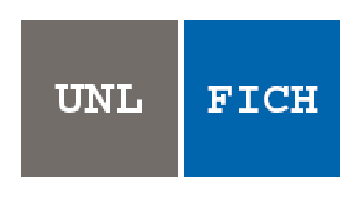
\includegraphics[scale=0.6]{img/fich_unl.eps}}
	\end{figure}
	
  	{Ingeniería Informática}\\
  	{Facultad de Ingeniería y Ciencias Hídricas}\\
    {UNIVERSIDAD NACIONAL DEL LITORAL}	
\end{center}

\bigskip
\bigskip

\newpage
\tableofcontents
\newpage
\pagestyle{plain}
\section{Métodos de extracción de características en imágenes parte 2}
\label{extraccion_caracteristicas}
Para aplicar el método SURF descripto en el informe anterior, se utiliza el código que ofrece la librería OpenCV (Open Source Computer Vision)\footnote{\url{http://SourceForge.net/projects/opencvlibrary}}. La funci\'on que lo implementa est\'a descrita a continuaci\'on:

\begin{lstlisting}
void cvExtractSURF(const CvArr* image, 
		   const CvArr* mask, 
		   CvSeq** keypoints, 
		   CvSeq** descriptors, 
		   CvMemStorage* storage, 
		   CvSURFParams params)
\end{lstlisting}

\noindent los parámetros\footnote{\url{http://opencv.willowgarage.com/documentation/feature_detection.html#cvExtractSURF}} de est\'a funci\'on son los que se presentan a continuación:
\begin{itemize}
 \item \textbf{image} (entrada): imagen de entrada en escala de grises de 8 bits.
 \item \textbf{mask} (entrada opcional): máscara de 8 bits. Las características sólo son buscadas en áreas que contienen más de un 50\% de los píxeles distintos de cero.
  \item \textbf{keypoints} (salida): puntero doble a una secuencia que representa los puntos claves. La secuencia de la estructura CvSURFPoint es la siguiente:
\begin{lstlisting}
typedef struct CvSURFPoint {
   CvPoint2D32f pt;
   int laplacian;
   int size;
   float dir;
   float hessian;
} CvSURFPoint;
\end{lstlisting}
donde:
\begin{description}
\item \texttt{pt:} es la posición de la característica en la imagen.
\item \texttt{laplacian:} representa el signo del laplaciando en el punto, los valores posibles son: -1, 0 o +1. Puede ser usado para la comparación de características (normalmente características con laplacianos de diferentes signos no coincidirán).
\item \texttt{size:} es el tamaño de la característica.
\item \texttt{dir:} es la orientación de la característica (0-360 grados).
\item \texttt{hessian:} es el valor del hessiano (puede ser usado para estimar aproximadamente la intensidad de las características). Relacionado con \texttt{params.hessianThreshold}.
\end{description}

\item \texttt{descriptors} (salida opcional): puntero doble a una secuencia que representa el descriptor. 
Dependiendo del valor de \emph{params.extended}, cada elemento de la secuencia contendrá un vector de punto flotante (CV\_32F) de 64 o 128 elementos. Si el parámetro es NULL, el descriptor no es calculado.
\item \texttt{storage}: almacenamiento de memoria donde serán guardados los puntos claves y descriptores.
\item \texttt{params}: otros parámetros del algoritmo con la estructura de CvSURFParams:
\begin{lstlisting}
typedef struct CvSURFParams
{  int extended;
   double hessianThreshold;
   int nOctaves;
   int nOctaveLayers;
} CvSURFParams;

CvSURFParams cvSURFParams(double hessianThreshold,
			  int extended=0);
\end{lstlisting}
donde:
\begin{description}
\item \texttt{extended:} tama\~no del descriptor. 0 indica un descriptor básico (64 elementos), mientras que 1 significa un descriptor extendido (128 elementos).
\item \texttt{hessianThreshold:} umbral para el hessiano del punto clave de las características, se extraen s\'olo aquellas cuyo hessiano supere el umbral.
% solamente las características con el hessiano del punto clave mayor a este valor serán extraídos. 
Los valores recomendables por defectos est\'an entre 300 y 500 (dependen del promedio local de contraste y nitidez de la imagen). 
%Con este parámetro se pueden filtrar ciertas características basadas en el valor del hessiano y otras características.
\item \texttt{nOctaves:} es el número de octavas a ser usadas en la extracción. Con cada octava adicional, el número de características es duplicado. (3 por defecto).
\item \texttt{nOctaveLayers:} es el número de capas en cada octava. (4 por defecto).
\end{description}
El objetivo de la función \emph{cvExtractSURF} es buscar características robustas en la imagen, como se ha descripto en el informe anterior y en \cite{Bay:2008:SRF}. Por cada característica hallada retorna su localización, tamaño, orientación y opcionalmente el descriptor (básico o extendido). Su uso puede ser la localización y seguimiento de objetos, emparejamiento de imágenes, entre otras aplicaciones.

\end{itemize}


\section{Correspondencia de características entre imágenes} %(Algoritmo knn - k-nearest neighbor algorithm).
Una vez que han sido identificados los puntos claves y sus descriptores asociados sobre la imagen, % utilizando las herramientas descriptas en la sección %(\ref{extraccion_caracteristicas}), 
se procede con la búsqueda de correspondencia (en caso de existir) entre la imagen patrón y la imagen del flujo de vídeo. De esta forma se busca identificar si el objeto está presente en la imagen capturada. 

Como se ha visto, un descriptor SURF \cite{Bay:2008:SRF, Bay:2008:SRF} es un vector de 64 dimensiones que caracteriza localmente una vecindad de un punto. 
En una aplicación típica, gran cantidad de descriptores SURF son extraídos de la imagen y la consulta consiste en buscar los vectores que mejor coincidan, entre los de la imagen objeto y los de la imagen del flujo de video.
Para ello, existen diversas técnicas, entre las cuales se presenta la denominada \textit{búsqueda del vecino más cercano} (del ingl\'es, Nearest Neighbor Search o NNS) \cite{AryaEtAl98}.

\subsection{Búsqueda del vecino más cercano}
El m\'etodo de búsqueda del vecino más cercano es de utilidad en una gran variedad de aplicaciones como el reconocimiento de imágenes, la compresión de datos, el reconocimiento de patrones y su clasificación, el aprendizaje máquina, los sistemas de recuperación de documentos, estadísticas y análisis de datos, entre otros. 

El método de la búsqueda del vecino más cercano, es un problema de optimización que intenta buscar los puntos más cercanos en un espacio métrico. Éste, puede definirse de la siguiente forma: dado un conjunto de puntos $P=\left\{ p_{1,...,}p_{n}\right\}$ en un espacio métrico $M$ y un punto de consulta $q \in M$, encontrar el/los punto/s más cercano/s a $q$ en $P$ donde $M$ es un espacio euclídeo d-dimensional y las distancia es medida mediante la distancia euclídea o Manhattan. 

Resolver este tipo de problemas no resulta trivial en espacios de grandes dimensiones, además no es usual encontrar algoritmos que posean un rendimiento mayor al de la búsqueda lineal (también conocida como ``búsqueda por fuerza bruta''), la cual resulta ser muy costosa y aveces inaplicable para muchas aplicaciones. Es por esto, que se ha generado un gran interés en algoritmos \footnote{\url{http://www.cs.umd.edu/~mount/ANN/}} que puedan realizar la búsqueda del vecino más cercano de forma aproximada, con lo cual es posible lograr mejoras significativas en tiempo de ejecución con errores de precisión relativamente pequeños \cite{Beis:1997:SIU:794189.794431} .

Existe una extensa variedad de publicaciones \cite{Muja09fastapproximate, AryaEtAl98, Beis:1997:SIU:794189.794431, conf/nips/LiuMGY04} que abordan el algoritmo de búsqueda del vecino más cercano de forma aproximada, en los que su rendimiento, varía dependiendo de las propiedades del conjunto de datos, tales como: la dimensionalidad, correlación y características de agrupación y tamaño. 
Uno de los algoritmos más usados para la búsqueda del vecino más cercano es KD-tree \cite{Beis:1997:SIU:794189.794431, friedman-an-algorithm-toms-77} (básicamente se trata de un árbol binario balanceado de búsqueda), el cual ha dado buenos resultados para la búsqueda exacta en datos de bajas dimensiones. Este algoritmo, ha sido modificado en diversos trabajos \cite{bb23918, AryaEtAl98, Beis:1997:SIU:794189.794431, VLDB95574, Fukunaga75, bb78856, bb79759, conf/nips/LiuMGY04, bb77826} para lograr reducir los tiempos de ejecución con datos de grandes dimensiones, a coste de obtener resultados aproximados. En el trabajo de Slipa-Anan y Hartley \cite{Silpa_KDTree, bb77826}, se propuso el uso de múltiples árboles KD aleatorios conocidos por su término en inglés como \textbf{Randomized KD-Tree}, donde se ha encontrado que dicho método, obtiene resultados satisfactorios en un amplio rango de problemas \cite{Muja09fastapproximate}.

\subsubsection{K-vecinos más cercanos}
Existe una variante al algoritmo NNS denominada k-NN (k-Nearest Neighbor). A diferencia del anterior, se debe especificar un parámetro K que establece cuantos vecinos influencian la clasificación de un punto. 
Estos vecinos son definidos utilizando una distancia métrica, por ejemplo la euclídea. 
Así, en el caso $K=1$ se está en presencia del algoritmo NNS. 
Si $K>1$ se utilizan los $K$ vecinos m\'as pr\'oximos al punto y se lo clasifica como perteneciente a la clase mayoritaria. 
% de tipo 
% ``lazy learning''(no usa el conjunto de datos de entrenamiento para hacer alguna generalización, en otras palabras, no hay una fase explícita de entrenamiento, o la misma es mínima) y no paramétrico (no se hace ninguna suposición sobre la distribución de los datos). La falta de generalización significa que KNN mantiene todos los datos de entrenamiento. Knn construye las decisiones basandose en todo el conjunto de datos (o en el mejor de los casos, en un subconjunto de los mismos).

%Se presenta una dicotomía aquí: si bien no existe una fase de entrenamiento, es costosa (en términos de tiempo y memoria) la fase de consultas.

% Suposiciones de KNN:
% 
% KNN supone que los datos están en un espacio característico. Más precisamente un espacio métrico. Los datos pueden ser escalares o vectores multidimensionales. Debido a que los puntos se encuentran en un espacio, estos tienen una noción de distancia (eg. la distancia euclidea).

% Cada uno de los datos de entrenamiento consiste en un conjunto de vectores con sus clases asociadas con cada vector(Que rempresentaría en mi las clases)

% \section{Nearest Neighbor search - wikpedia}
% Nearest neighbor search(NNS), también conocido como búsqueda de proximidad, búsqueda por similitud o búsqueda del más cercano, es un problema de optimización que intenta encontrar los puntos más cercanos en un espacio métrico. Esto es: dado un conjunto $S$ de puntos en un espacio métrico $M$ y un conjunto de puntos $q$ de consulta (con $q \in M$), encontrar el punto más cercado en $S$ para $q$. En muchos casos, $M$ se toma como un espacio euclídeo d-dimensional y la distancia se mide por la distancia euclídea o la distancia Manhattan.

%\subsection{FLANN - Fast Library for Approximate Nearest Neighbors - Fast approximate nearest neighbors with automatic algorithm configuration}

%\subsection{Investigaciones previas}
\subsection{El algoritmo de árboles KD aleatorio}
Como se mencionó anteriormente, el algoritmo KD-tree clásico \cite{friedman-an-algorithm-toms-77} resulta eficiente con datos de bajas dimensiones, pero su rendimiento se ve afectado rápidamente al aumentar la dimensionalidad. 
Para obtener una velocidad mayor a la de la búsqueda lineal se hace necesario establecer una búsqueda aproximada del vecino más cercano. Esto mejora el tiempo de búsqueda pero, como contrapartida, el algoritmo no siempre da como resultado el vecino más cercano.

Los elementos guardados en el árbol KD-tree, son vectores de altas dimensiones. En el primer nivel (la raíz del árbol), los datos son divididos en dos mitades por un hiper plano ortogonal a una dimensión elegida con un valor de umbral. Generalmente, esta división se realiza con la media, en la dimensión con la mayor varianza del conjunto de datos. Se utiliza la media ya que con características visuales provistas por SIFT o SURF, es la medida que presenta el mejor rendimiento \cite{Muja09fastapproximate}. Mediante la comparación del vector de consulta con el ``valor de partición'', es fácil determinar a que mitad del conjunto de datos pertenece el vector de consulta. 
Cada una de las mitades de los datos es dividida de igual manera y en forma recursiva, para lograr crear un árbol binario completamente balanceado. 
Cada nodo de la parte inferior del \'arbol corresponde a un punto simple del conjunto de datos. 
Sin embargo, en algunas aplicaciones los nodos hojas pueden tener más de un punto.

Slipa-Anan y Hartley han propuesto una versión del algoritmo de árbol KD en el que múltiples árboles KD aleatorios son creados \cite{Silpa_KDTree, bb77826}. El algoritmo de árboles KD original, divide los datos por la mitad en cada nivel del árbol sobre la dimensión para la cual los datos exhiben la mayor varianza. 
A diferencia de \'estos, los árboles aleatorios son construidos seleccionando la dimensión de división 
de forma aleatoria, sobre las primeras $D$ dimensiones en las que los datos tienen mayor varianza. 
Se usa el valor fijo $D=5$ que resulta el más adecuado para diferentes datos \cite{Muja09fastapproximate}. %Un ajuste adicional sobre dicho valor, no otorga beneficios importantes.

Cuando se realiza la b\'usqueda en el árbol, una cola con prioridad es mantenida a través de todos los arboles aleatorios, por lo que la búsqueda estará ordenada mediante el incremento de la distancia a cada nodo del borde. 
El grado de aproximación, se determina mediante el examen de un número fijo de nodos hoja, en cuyo momento la búsqueda termina y devuelve los mejores candidatos.

%using PCA would result in better splits, but it's significantly more expensive and in the end the cost is bigger than the benefit.
%  En la implementación FLANN \cite{Muja09fastapproximate}, el usuario especifica solamente la precisión de búsqueda deseada, la que es usada durante el entrenamiento para seleccionar el número de nodos hojas que deben ser examinados, con el objetivo de alcanzar dicha precisión.
%por defecto esta chequeando 32 hojas....

Se debe tener en cuenta que la cantidad de memoria utilizada aumenta linealmente con el número de árboles aleatorios, una característica poco feliz y cuya importancia no resulta menor a la hora de monitorizar la sobrecarga del sistema.


% La precisión del método, es mayor cuando se utilizan parches de imágenes como pruebas, en vez de usar números aleatorios, ya que en los primeros existe una alta probabilidad de que los datos estén correlacionados.

% (en \cite{flann_visapp09} se evaluan varios algoritmos mostrando los resultados y su velocidad respecto a la busqueda lineal, en el que kd-trees da buenos resultados. Tener en cuenta que en nuestro caso tenesmos n keypoints * 64 elementos (eso nos da el total de dimensiones) => es muy dificil que llegue a los 15k puntos de keypoints detectados ya que por el umbral que le metemos en la detecció nunca saca tantos.. y recién a partir de tener 1000000 de dimenesiones es donde el randomized kd-tree se hace muy lento.....
%a diferencia de los kmeans por ejemplo, el método de kd-tree es más rápido pero menos preciso.)
 
%1 - porque se hace la construcción del arbol sobre los datos capturados sobre cada frame y no sobre la imágen a detectar?
%2 - en el paper de la implementación de flann los datos que se usan son distintos a los míos ya que difieren tanto las dimenesiones como la cantidad de puntos. - cantidad de arboles a usar, cantidad de hojas a utilizar.
%3- checkeo de knn con k=2 se chequean 2 vecinos y el que esta mas cerca es el que agarra?
%4- 

%%K-nearest neighbor (KNN) queries: “find the K-most similar objects in the database with respect to a given object”.

%%pagina 99 y 104 de libro nestor comp grafica DeBerg.... =>kdtree y randomized binary search tree


% \subsection{optimised kd-trees for fast images descriptor matching}
% Los descriptores obtenidos mediante la aplicación del método SURF a una imagen son N vectores de 64 dimensiones, donde N representa el número de puntos claves detectados.
% 
% La consulta consiste en buscar el vector descriptor de la imagen objeto que más se asemeja al vector descriptor de la imagen live.

%%%%%%%%%%%%%%%%%%%%%%%%%%%%%%%%%%%%%%%%%%%%%%%%%%%%%%%%%%%%%%%%%%%%%%%%%%%%%%%%%%%%%%%%%%%%%%
%%%%%%%%%%%%%%%%%%%%%%%%%%%%%%%%%%%%%%%%%%%%%%%%%%%%%%%%%%%%%%%%%%%%%%%%%%%%%%%%%%%%%%%%%%%%%%
\subsection{Búsqueda de correspondencia - Implementación}
La librería Rápida para aproximación de vecinos más cercanos (FLANN - Fast library for Approximate Nearest Neighbors) \cite{Muja09fastapproximate}, contiene una colección de algoritmos optimizados para la búsqueda rápida del vecino más cercano, en grandes conjuntos de datos y con  características de altas dimensiones.
OpenCV, posee una interfaz\footnote{\url{http://opencv.willowgarage.com/documentation/cpp/flann_fast_approximate_nearest_neighbor_search.html}} a la librería FLANN\footnote{\url{http://people.cs.ubc.ca/~mariusm/index.php/FLANN/FLANN}} la cual ser\'a utilizada para poder resolver el problema de la búsqueda. 
A continuación se presenta una descripción de los principales métodos de FLANN.

La clase index de FLANN se utiliza para abstraer los diferentes tipos de índices a usar para las búsqueda del vecino más cercano.
\begin{lstlisting}
namespace cv
{
namespace flann
{
    template <typename T>
    class Index_
    {
    public:
            Index_(const Mat& features, const IndexParams& params);
            ~Index_();
            ...
            void knnSearch(const Mat& queries,
                           Mat& indices,
                           Mat& dists,
                           int knn,
                           const SearchParams& params);
	    ...
            const IndexParams* getIndexParameters();
    };
    typedef Index_<float> Index;
} } // namespace cv::flann
\end{lstlisting}
El constructor de la clase
\begin{lstlisting}
Index_<T>::Index_(const Mat& features, const IndexParams& params)
\end{lstlisting}
construye un índice de búsqueda del vecino más cercano para un conjunto de datos dado. Los parámetros
\footnote{ \url{http://opencv.willowgarage.com/documentation/cpp/flann_fast_approximate_nearest_neighbor_search.html#cv::flann::Index_} }
son:
\begin{itemize}
  \item \textbf{features:} matriz que contiene las características (puntos) a indexar. Se almacena un punto por cada fila de la matriz; el tamaño de la matriz es $C$x$D$, donde $C$ es la cantidad de caracter\'isticas y $D$ es la dimensionalidad.
  \item \textbf{params:} estructura que contiene los parámetros del índice. El tipo del índice será construido dependiendo del tipo de este parámetro. Los parámetros\footnote{\url{http://opencv.willowgarage.com/documentation/cpp/flann_fast_approximate_nearest_neighbor_search.html#id4}} posibles son:
  \begin{itemize}
    \item \textbf{LinearIndexParams}: el índice lleva a cabo una búsqueda de fuerza bruta lineal.
    \item \textbf{KDTreeIndexParams}: el índice construido consiste en un conjunto de árboles aleatorios KD (randomized KD-trees) que se buscará en paralelo.
	\begin{lstlisting}
	      struct KDTreeIndexParams : public IndexParams{
		  KDTreeIndexParams( int trees = 4 );
	      };
	\end{lstlisting}
	\textbf{trees:} el número de árboles KD paralelos a usar. Valores que producen buenos resultados se encuentran entre 1 y 16, dependiendo del conjunto de datos.
    \item \textbf{KMeansIndexParams}: el índice construido será un árbol k-means jerárquico.
    \item \textbf{CompositeIndexParams}: el índice creado combina árboles aleatorios KD y k-means jerárquicos.
    \item \textbf{AutotunedIndexParams}: el índice creado será seleccionado automáticamente para ofrecer el mejor rendimiento eligiendo el tipo de índice óptimo entre el uso de árboles aleatorios KD, k-means jerárquicos o lineales, como así también, los parámetros para el conjunto de datos proporcionados.
    \item \textbf{SavedIndexParams}: este tipo de objeto es usado para cargar un índice previamente guardado en el disco.
  \end{itemize}
\end{itemize}

La funci\'on \textbf{knnSearch} lleva a cabo la búsqueda de los K-vecinos más cercanos para un punto dado, usando el índice. A continuación se presentan los parámetros\footnote{\url{http://opencv.willowgarage.com/documentation/cpp/flann_fast_approximate_nearest_neighbor_search.html#cv-cv-flann-index-t-knnsearch } } 
de dicha función:
\begin{lstlisting}
void Index_<T>::knnSearch(const Mat& queries, 
			  Mat& indices, 
			  Mat& dists, 
			  int knn, 
			  const SearchParams& params)
\end{lstlisting}
Parámetros:
\begin{itemize}
  \item \textbf{query:} matriz con puntos para realizar la consulta, su tamaño es $C$x$D$, donde $C$ es la cantidad de caracter\'isticas y $D$ es la dimensionalidad (un punto por fila).
  \item \textbf{indices:} matriz que contendrá los índices de los K vecinos más cercanos encontrados.
  \item \textbf{dists:} matriz que contendrá las distancias a los K vecinos más cercanos encontrados.
  \item \textbf{knn:} número de vecinos más cercanos para los que se hará la búsqueda.
  \item \textbf{params:} parámetros de búsqueda
\begin{lstlisting}
 struct SearchParams {
        SearchParams(int checks = 32);
};
\end{lstlisting}
\textbf{checks:} especifica las hojas máximas a visitar en la búsqueda de los vecinos. Un valor alto para este parámetro, dará una mejor precisión, pero requerir\'a más tiempo. Si se utilizó la configuración automática cuando se creó el índice, el número de controles necesarios para alcanzar la precisión especificada también fue calculado, en cuyo caso se omite este parámetro.
\end{itemize}

% poner aca que corno utilizamos d ela librería y con que parámetros....

%\section{slipa modificado por mi}

% 
% \subsection{esquema de búsqueda en árbol kd}
% La idea general detrás de los árboles KD se describirá a continuación. Los elementos guardados en el árbol KD son vectores de altas dimensiones en $R^d$. En el primer nivel (la raíz) del árbol, los datos son divididos en dos mitades por un hiper plano ortogonal a una dimensión elegida con un valor de umbral. Generalmente, esta división sea realiza se realiza con la media en la dimensión con la mayor varianza del conjunto de datos. Mediante la comparación del vector de consulta con el ``valor de partición'', es fácil determinar a que mitad de el conjunto de datos del vector de consulta pertenece. Cada una de las mitades de los datos, es luego recursivamente dividida de la misma forma explicada anteriormente para crear un árbol binario completamente balanceado.
% En la parte inferior del árbol, cada nodo del árbol, corresponde a un punto simple del conjunto de datos, aunque en algunas aplicaciones, los nodos hojas pueden tener más de un punto.
% La profundidad del árbol resulta ser $log_2 (N)$ donde $N$ es el número de puntos del conjunto de datos.

% Dado un vector de consulta, un descenso en el árbol requiere $log_2(N)$ comparaciones y el acceso a un nodo hoja del arbol.


%\section{knn search}
%http://saravananthirumuruganathan.wordpress.com/2010/05/17/a-detailed-introduction-to-k-nearest-neighbor-knn-algorithm/


%%%%%%%%%%%%%%%%%%%%%%%%%%%%%%%%%%%%%%%%%%%%%%%%%%%%%%%%%%%%%%%%%%%%%%%%%%%%%%%%%%%%%%%%%%%%%%%%%%%%%%%%%%%%
%%%%%%%%%%%%%%%%%%%%%%%%%%%%%%%%%%%%%%%%%%%%%%%%%%%%%%%%%%%%%%%%%%%%%%%%%%%%%%%%%%%%%%%%%%%%%%
\newpage
\bibliographystyle{alpha}
\bibliography{bib1,bib2,bib3,bib4}
 \end{document}
